\documentclass{article}
\usepackage{tikz}
\usetikzlibrary{shapes.geometric}

\begin{document}

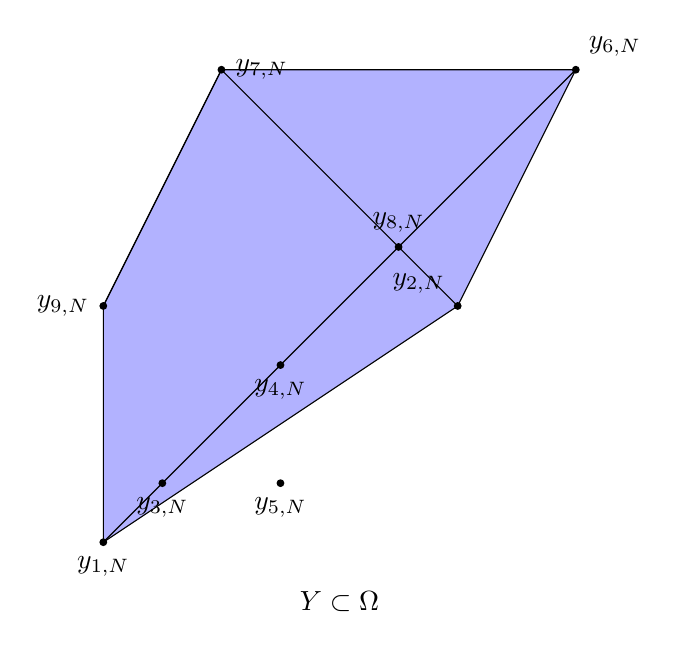
\begin{tikzpicture}[scale=1.5]
    % Define the vertices of the polygon
    \coordinate (A) at (0,0);
    \coordinate (B) at (3,2);
    \coordinate (C) at (4,4);
    \coordinate (D) at (1,4);
    \coordinate (E) at (0,2);

    % Draw the polygon
    \draw[fill=blue!30] (A) -- (B) -- (C) -- (D) -- (E) -- cycle;

    % Draw the diagonals to form triangles
    \draw (A) -- (C);
    \draw (B) -- (D);
    \draw (E) -- (D);

    % Label the vertices
    \node at (A) [circle,fill,inner sep=1pt,label=below:$y_{1,N}$] {};
    \node at (B) [circle,fill,inner sep=1pt,label=above left:$y_{2,N}$] {};
    \node at (C) [circle,fill,inner sep=1pt,label=above right:$y_{6,N}$] {};
    \node at (D) [circle,fill,inner sep=1pt,label=right:$y_{7,N}$] {};
    \node at (E) [circle,fill,inner sep=1pt,label=left:$y_{9,N}$] {};

    % Label the quadrature nodes
    \node at (0.5,0.5) [circle,fill,inner sep=1pt,label=below:$y_{3,N}$] {};
    \node at (1.5,1.5) [circle,fill,inner sep=1pt,label=below:$y_{4,N}$] {};
    \node at (2.5,2.5) [circle,fill,inner sep=1pt,label=above:$y_{8,N}$] {};
    \node at (1.5,0.5) [circle,fill,inner sep=1pt,label=below:$y_{5,N}$] {};

    % Label the domain and its subset
    \node at (2,-0.5) {$Y \subset \Omega$};
\end{tikzpicture}

\end{document}